\documentclass[Bachelorarbeit.tex]{subfiles}
\begin{document}
\chapter{Implementierung}
\label{chap:implementierung}

\section{Spezifikation}
\label{chap:implementierung:sec:spezifikation}
Wie zuvor im Kapitel \nameref{chap:entwicklung} schon definiert wurde soll der Prototyp, in Form einer Web-Applikation, in die bestehende Lösung Pery integriert werden.
Dadurch kann, aufgrund der Abhängigkeit zu Pery, nur eine vollständige Kompatiblität zu der aktuellen Versionen des Webbrowsers Mozilla Firefox und Google Chrome gewährleistet werden.   
Im Zuge der vorangegangen Analysen, sowie verschiedenen Rahmenbedingung werden die nachfolgenden Technologien für die Implementierung eingesetzt. 

\subsection*{Programmiersprachen}
Grundsätzlich wird der Prototyp auf Serverseite mit Python in der Version 2.7 realisiert. 
Dabei handelt es sich viel mehr um eine Vorgabe, da der Prototyp innerhalb des bestehenden Systems Pery integriert wird. Pery selbst wird mithilfe des Webframeworks Django entwickelt, welches in Python geschrieben ist.
Bei Python handelt es sich um 
\ideas{kurze Info über Python und seine Besonderheiten}

Ergänzend zu Python wird clientseitig teilweise Java Script eingesetzt. 

\subsection*{Webframeworks}
Im speziellen spielen die Frameworks Django 
\ideas{Was ist Django und wie funktioniert es. Schwerpunkt auf: DB Abstraktion, Admin, View, Templates, Render Engine}

\ideas{nochmal kurz info zu Leaflet.js}

\section{Details zur Implementierung}
\label{chap:implementierung:sec:details}

\subsection{Implementierung Serverseite}
\label{implServer}
Anhand des Sequenzdiagrammes (siehe Abbildung \ref{fig:Overview}) soll ein  Überblick über den Standardablauf auf der Serverseite vermittelt werden. 
Sobald die Anwender\_innen im  Prototyp auf den Link edit trip klicken wird eine  Anfrage an den Webserver gesendet.
Der Webserver bereitet die erhaltenen Daten auf und leitet sie an die Admin-Seite des Trips (TripAdmin) weiter (siehe Abbildung \ref{fig:Overview} - request). 
Die Funktion Planning Trip Action des TripAdmins wird dabei aufgerufen und die entsprechende View (TripBase) geladen (siehe Abbildung \ref{fig:Overview} - initial TripBase).
Innerhalb der View werden bis zur Rücksendung der Antwort (Response) an den Web Server die drei Funktionen prepare, render\_output und render\_to\_response durchlaufen
Dabei wird in der Funktion prepare hauptsächlich die \ac{AJAX}-Funktionalität aktiviert.
Die benötigten Daten werden in der Funktion render\_output (siehe Absatz \nameref{renderOutput}) aus der Datenbank geladen und entsprechend vorbereitet bis sie anschließend an die Funktion render\_to\_response oder über das \ac{AJAX}-Framework (nicht in der Abbildung) an den Webserver weitergeleitet werden.
In der Funktion render\_to\_response werden die definierten Templates anhand der erhaltenen Daten, mithilfe des Django-Frameworks, in das \ac{HTML}-Format übertragen und in einen Response eingebettet.
Abschließend wird der generierte Response an den Webserver weitergegeben, der ihn schlussendlich an den Web Browser ausliefert.


\begin{figure}[h]
\centering
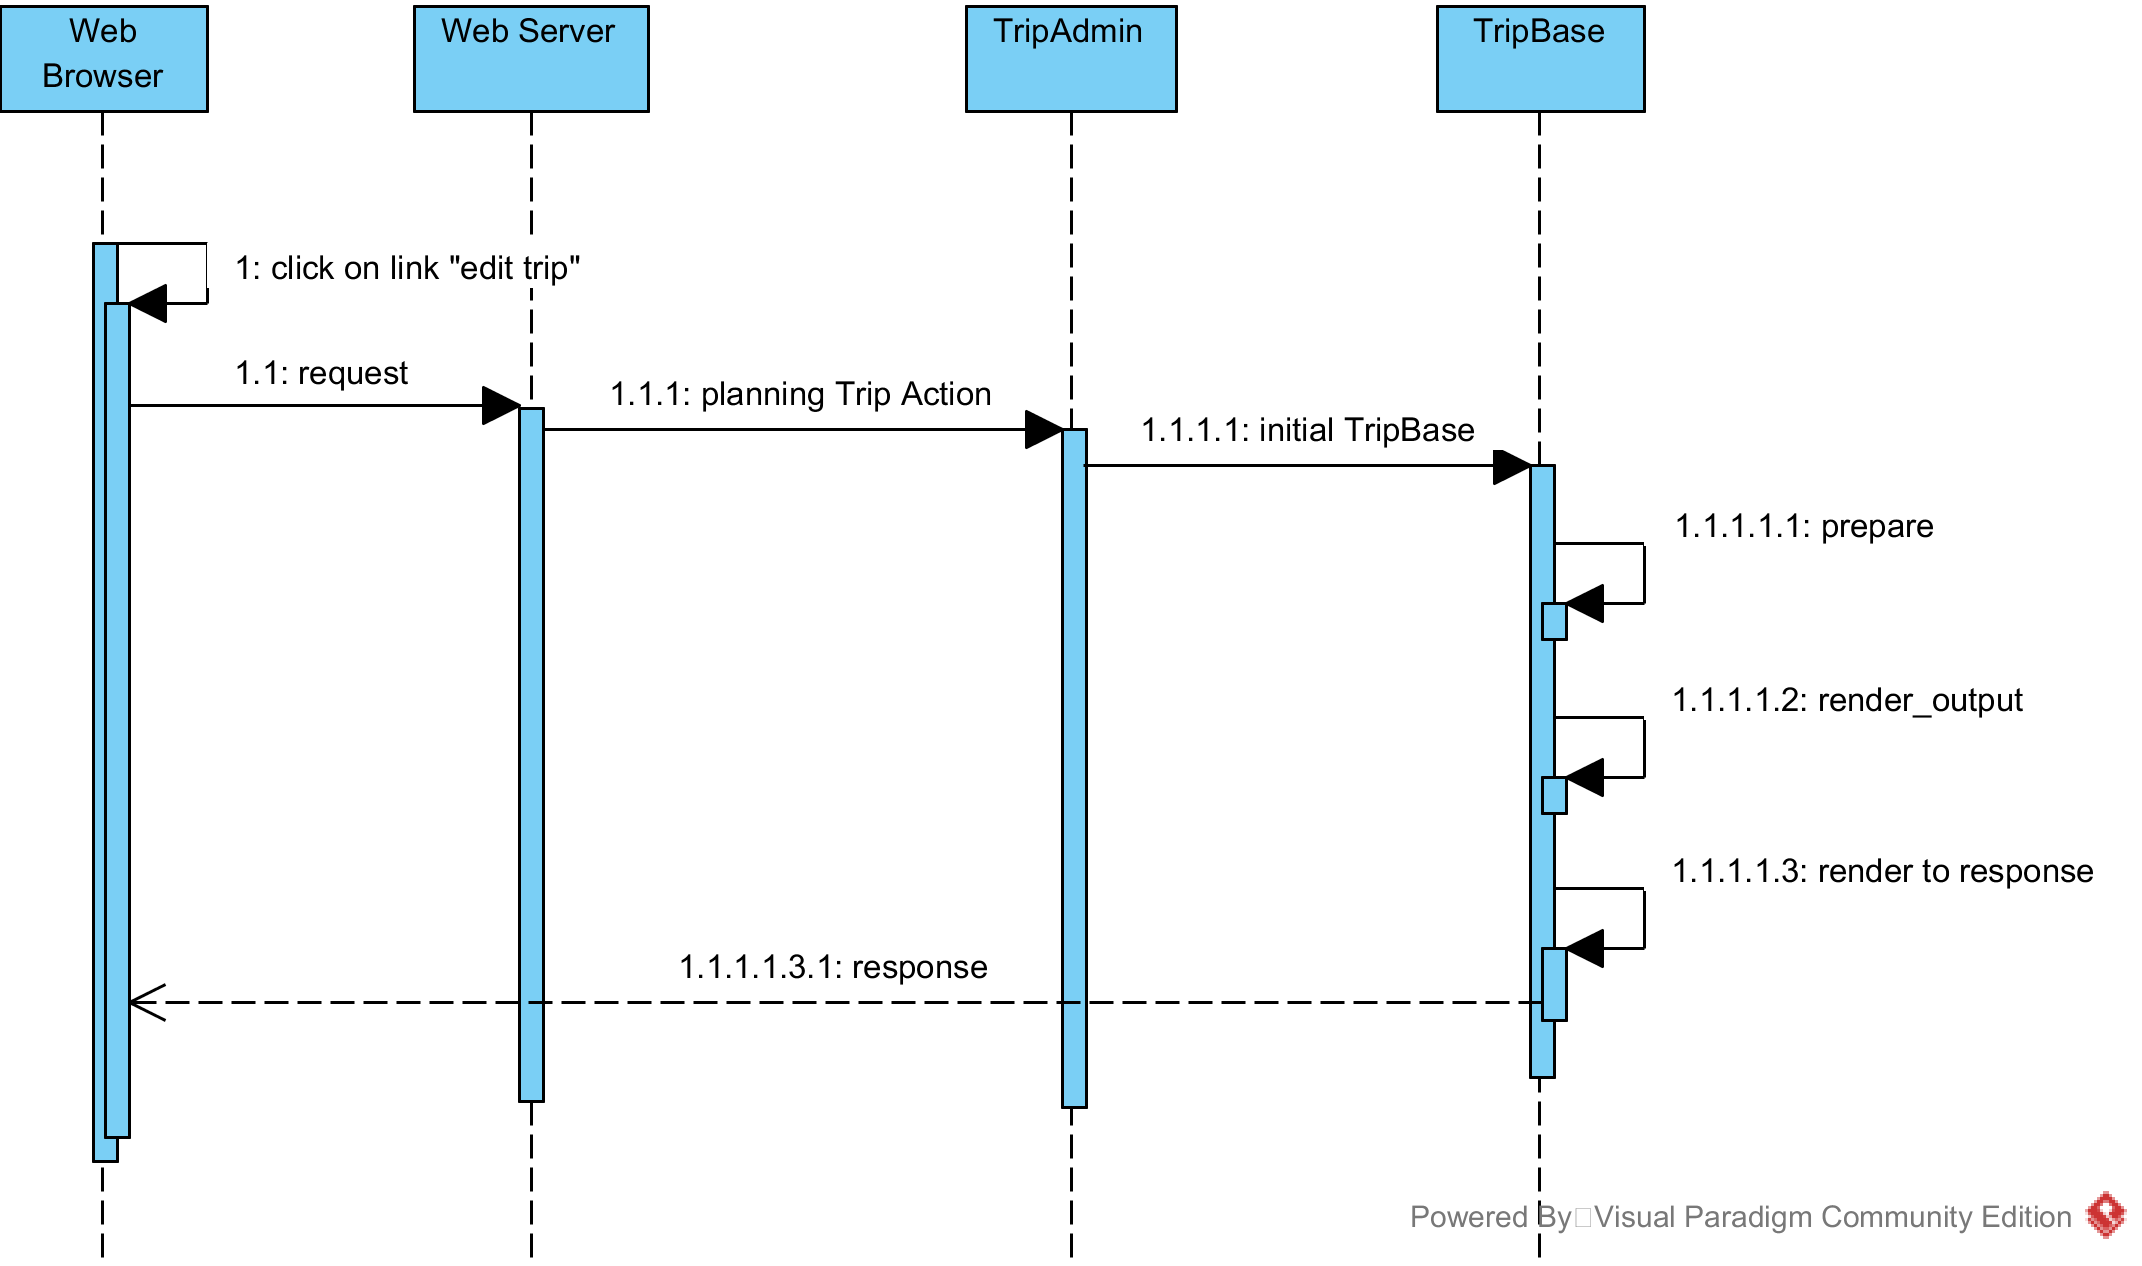
\includegraphics[width=1\linewidth]{img/Implementierung/Overview}
\caption[k]{Sequenzdiagramm: Übersicht des Ablaufs vom Request bist zum Response. Quelle: eigene Ausarbeitung.}
\label{fig:Overview}
\end{figure}

\subsubsection*{Funktion: render\_output}
\label{renderOutput}
Nachdem die Funktion prepare in der TripBase View abgeschlossen ist wird die Funktion render\_output gestartet (siehe Abbildung \ref{fig:Overview}).
Beginnend mit dem Auslesen des PresantationMode aus dem Request, welcher als Parameter übergeben wird, wird definiert ob die Karten oder Listenansicht erstellt werden soll (siehe Abbildung \ref{fig:renderOutput} - 1.).
Sollte das Auslesen nicht möglich sein, weil der Trip beispielsweise das erste Mal aufgerufen wird, so wird die Kartenansicht als Standartwert verwendet.
Sollte es sich bei dem Request um einen \ac{AJAX}-Aufruf handeln so wird dieser, je nach Bedarf abgewickelt und als Response an den Webserver zurück geschickt.
Anschließend werden mittels der Datenbankabstraktion alle Tripstations\footnote{Tripstations sind Unternehmen welche bereits dem Trip hinzugefügt wurden.} geladen (siehe Abbildung \ref{fig:Overview} - 2. bis 2.3).
An dieser Stelle teilt sich der weitere Ablauf auf, je nach dem welcher PresentationMode gewählt wurde und es sich nicht um einen \ac{AJAX}-Aufruf handelt (siehe Abschnitte \nameref{PERYMapTrip} und \nameref{PERYListTrip}).\\


\paragraph{Rank}
\label{Rank}
Im Vorfeld wurde definiert, dass die Marker der Karte durch die Verwendung unterschiedlicher Farben, zusätzliche Informationen zu den Unternehmen transportieren sollen. 
Dazu gehören beispielsweise der Gesamtumsatz oder der letzte Besuch, diese Kategorien werden als Rank bezeichnet.
Dafür müssen die Daten entsprechend vorbereitet und zur Verfügung gestellt werden.
\\
Um dies zu realisieren wurde die Klasse PeryDataRank geschrieben (siehe Abbildung \ref{fig:ClassDiagrammRank}). 
Innerhalb der View (TripBase), wird für jeden Rank ein Objekt der Klasse PeryDataRank erstellt (available\_ranks).
Dabei wird über die Attribute des Objektes (clazz:string und attr:string) gesteuert woher die Daten für diesen Rank kommen sollen. \\

\ideas{Stand Korrektur 10.11.2016}

\begin{figure}[H]
\centering
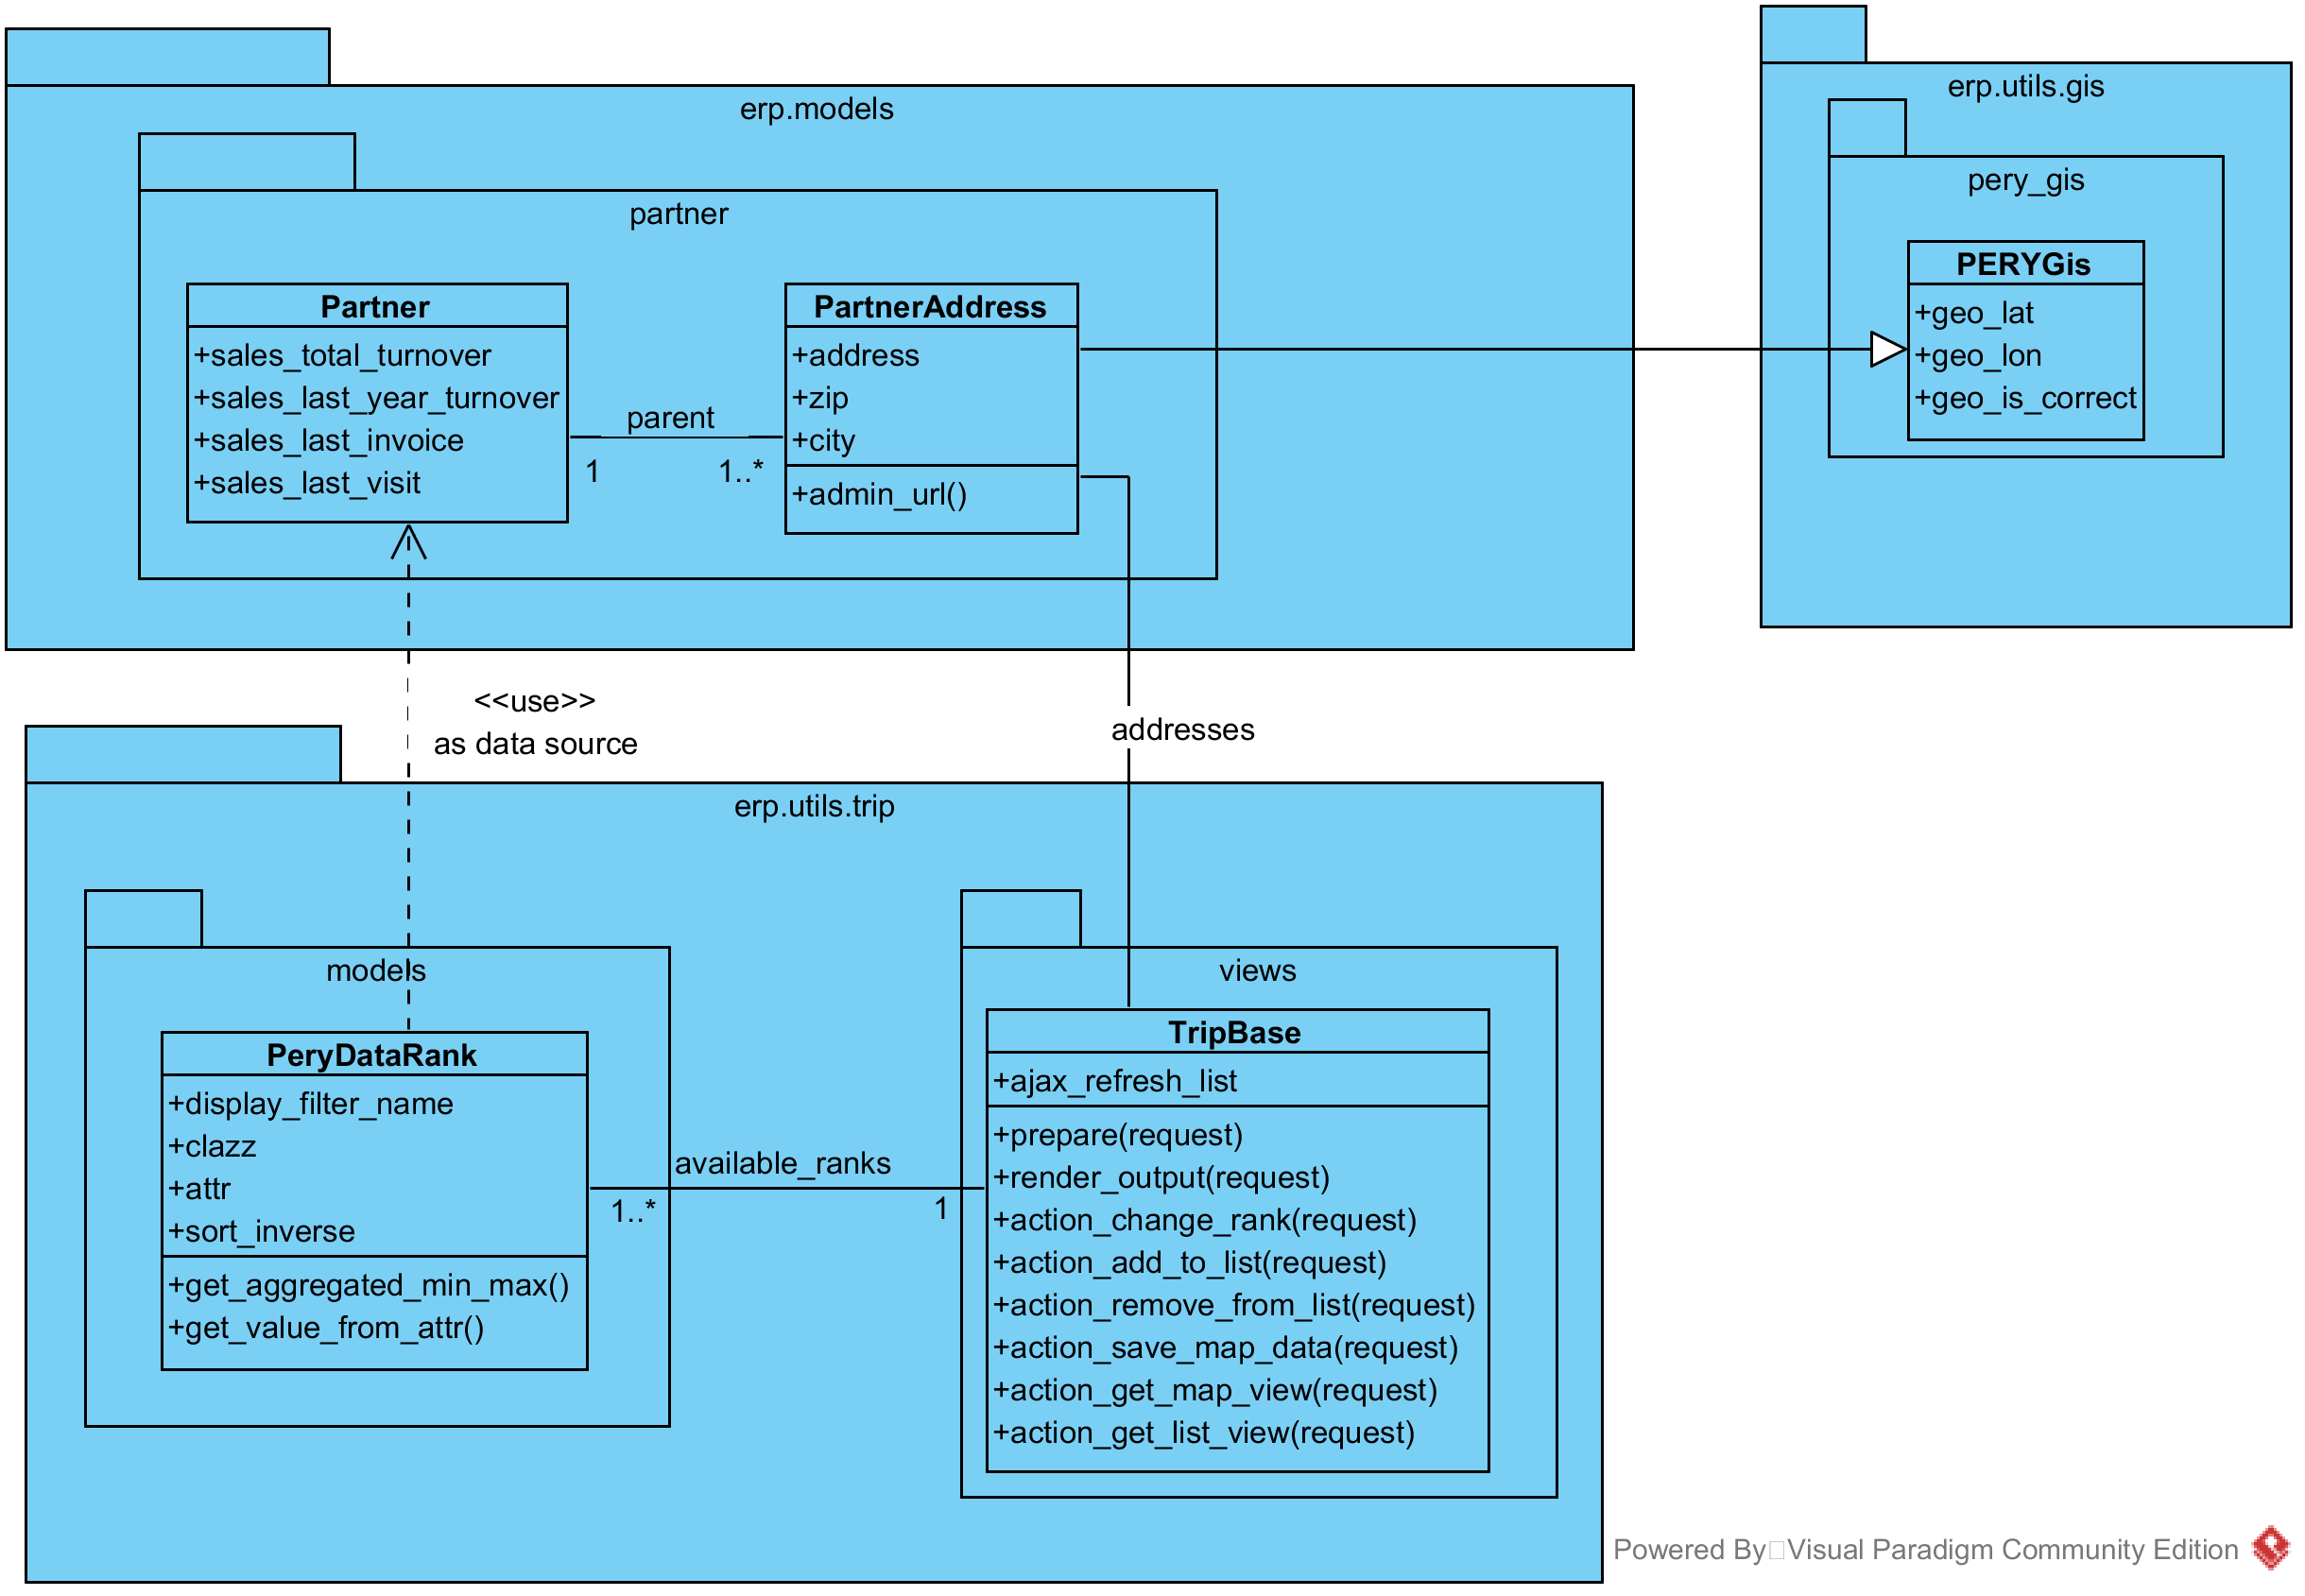
\includegraphics[width=0.9\linewidth]{img/Implementierung/ClassDiagrammRank}
\caption[k]{Klassendiagramm: PeryDataRank. Quelle: eigene Ausarbeitung.}
\label{fig:ClassDiagrammRank}
\end{figure}

Dabei ist anzumerken, dass die verfügbaren Ranks (available ranks), als Dictionary mit dem Datentyp PeryDataRank auf Klassenebene der View (TripBase) definiert werden.

\paragraph{PERYMapTrip}
\label{PERYMapTrip}
Im Fall der Kartenansicht wird ein Objekt der Klasse PERYTripMap initialisiert. 
Anschließend werden, mittels der Datenbankabstraktion alle Objekte der Klasse PartnerAddress geladen welche über Daten in den Attributen geo\_lat und geo\_lon verfügen (siehe Abbildung \ref{fig:Overview} - 4. bis 4.3). \\
\\
Um die Marker auf der Karte später nach dem ausgewählten Rank entsprechend einzufärben muss der Rank noch korrekt erstellt werden (siehe Abschnitt \nameref{Rank}). 
Dafür wird im ersten Schritt der aktive Rank aus den Request Parametern ausgelesen und verglichen ob er verfügbar ist.

Mittels einer Funktion wird aus dem aktiven PeryDataRank die entsprechenden min. und max. Werte (Bsp. letzter Besuch) aus dem dazugehörigen Partner Objekten
	\footnote{Auf die Partner Objekte wird über den Fremdschlüssel in dem PartnerAddress Objekt zugegriffen (siehe Abbildung \ref{fig:ClassDiagrammRank})}  
berechnet (siehe Abbildung \ref{fig:renderOutput} - 5.).
Anhand der berrechneten min. und max. Werte sowie der gegeben Anzahl an Abstufungen (Range) können nun Ranges eingeteilt und an die Karte (PERYTripMap) weitergegeben werden.
	\footnote{Beispiel: Der aktive Rank ist Gesamtumsatz. Dabei belaufen sich die min. und max. Werte auf 0 Euro bis 10.000 Euro, die Anzahl der Ranges entspricht 5. Somit fallen die Unternehmen mit einem Gesamtumsatz von 0 Euro bis 2000,00 Euro in Range 1, von 2000,01 Euro bis 4000,00 Euro in Range 2, ..., von 8000,01 Euro bis 10.000,00 Euro in Range 5.} 
Nun wird für alle PartnerAddress, welche zuvor aus der Datenbank gelesen wurden, jeweils die Funktion addPoint des PERYMapTrip  aufgerufen. 
Diese Funktion erzeugt im ersten Schritt einen neuen PeryMapPoint, welcher alle Informationen (Koordinaten, Daten für das Popup, etc.) besitzt die für die Visualisierung auf der Karte notwendig ist.
Im zweiten Schritt wird das neue Objekt klassifiziert.  
Anhand seines Rank-Wertes wird das Objekt in eine der zuvor definierten Ranges eingeteilt (siehe Abbildung \ref{fig:renderOutput} - 7. bis 7.3).

\paragraph{PERYListTrip}
\label{PERYListTrip}
Sollte die Listenansicht ausgewählt sein wird der vorhergehende Abschnitt durch diesen ersetzt.
Dabei wird im ersten Schritt ein Objekt der Klasse PERYListTrip in der View (TripBase) angelegt.
Anschließend werden die PartnerAddresses Objekte aus der Datenbank geladen und der Sammlung im PERYListTrip hinzugefügt (siehe Abbildung \ref{fig:renderOutput} - 9. bis 10.).



\begin{figure}[h]
\centering
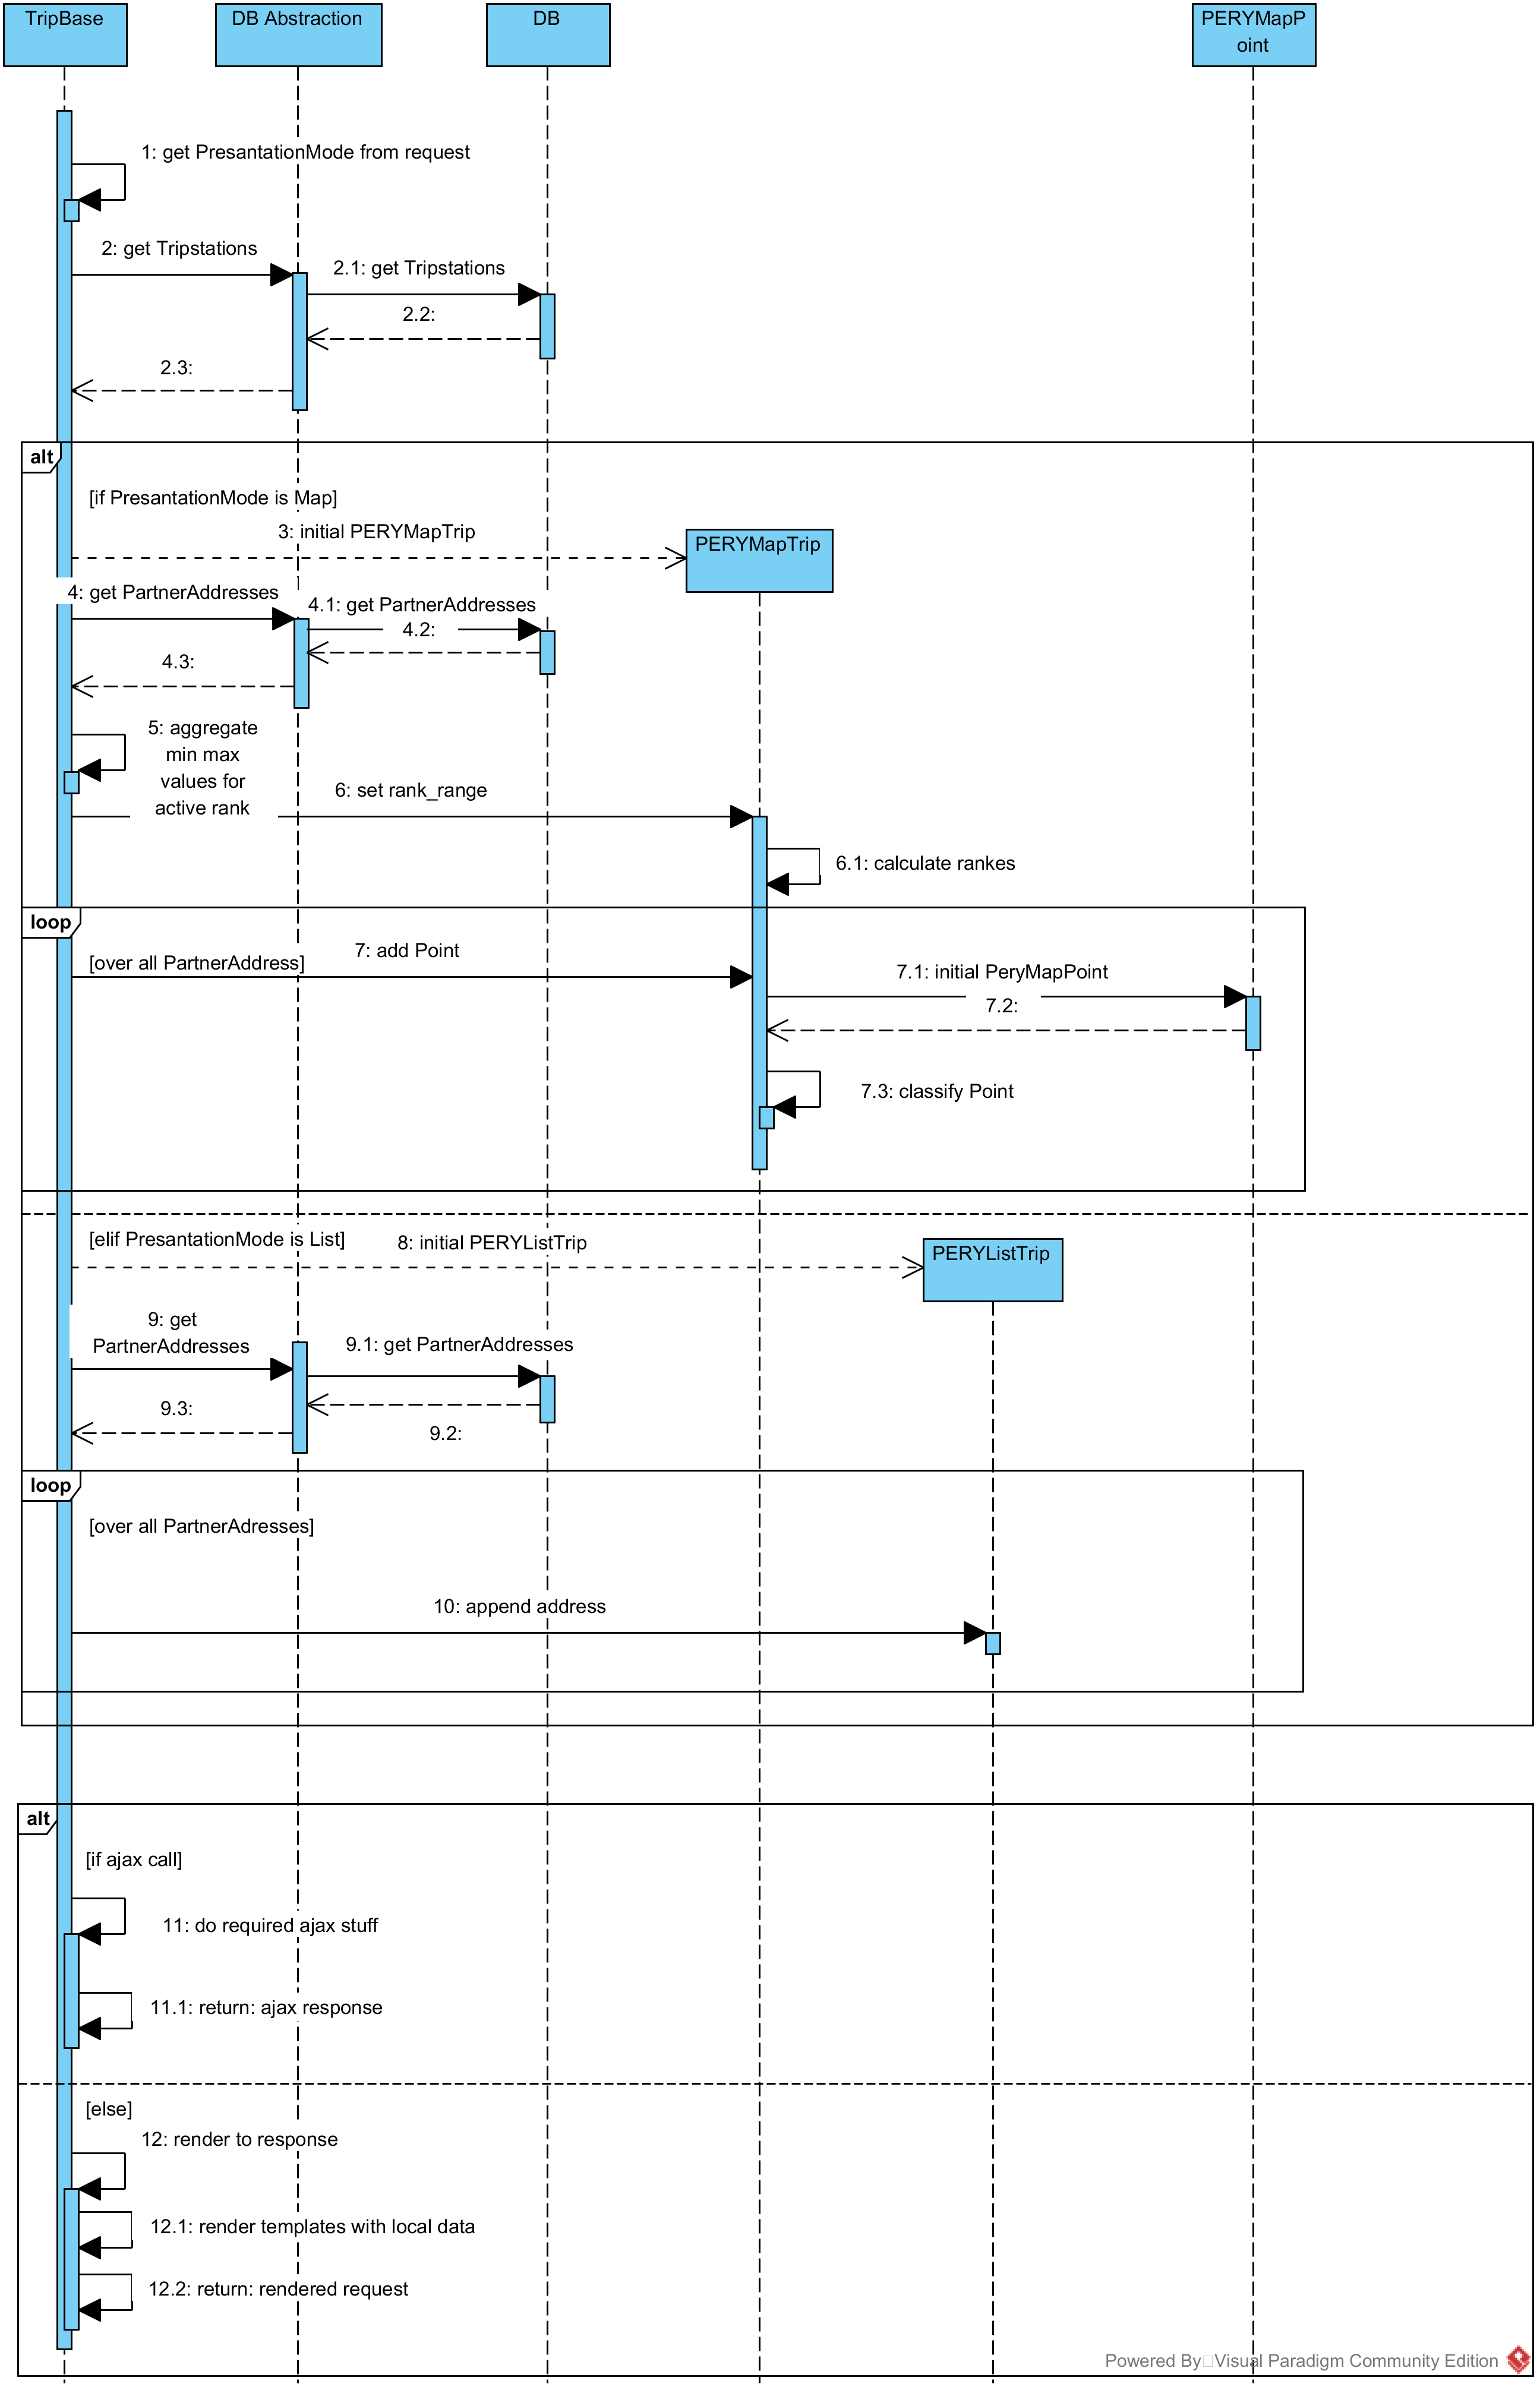
\includegraphics[width=1\linewidth]{img/Implementierung/renderOutput}
\caption[k]{Sequenzdiagramm: Ablauf der Funktion render\_output auf dem Server. Quelle: eigene Ausarbeitung.}
\label{fig:renderOutput}
\end{figure}

\subsection{Implementierung Clientseite}
Bei der Realisierung des Prototypen diente der zuvor angefertigte Mockup als Orientierung. 
Demnach wurde der Prototyp ebenfalls in die drei Teile Kopfbereich, Tripliste und Container für die diversen Ansichten unterteilt (siehe Abbildung \ref{fig:prototypMockup}).


\subsubsection*{Kopfbereich}
Wie zuvor im Prototyp erwähnt soll dieser Bereich der Orientierung und Navigation dienen.
Bei der Realisierung des Prototypen wird dabei die Vorlage des Mockups übernommen.
Im linken Bereich wird dargestellt welche Funktion des Prototypen gerade genutzt wird.
	\footnote{Aktuell ist für den Prototyp nur die Funktionalität Trips zu bearbeiten verfügbar.}
Im rechten Bereich ist der Button hinterlegt mit welchem zwischen der Karten- und Listenansicht gewechselt werden kann.

\subsubsection*{Tripliste}
Der linke Hauptbereich ist für die Tripliste reserviert.
Im oberen Teil wird der Name des zu bearbeitenden Trips angezeigt.
Wenn die Kartenansicht geöffnet ist, befindet sich im Fußbereich ein Button mit dem die Karte so eingestellt wird, das alle ausgewählten Unternehmen auf einen Blick sichtbar sind.
Die restliche Höhe des Browsers genutzt um, ähnlich wie im Mockup, die bereits ausgewählten Unternehmen, als separate Elemente innerhalb der Liste, darzustellen.
Wenn die Höhe des Browserfensters nicht ausreicht um alle Unternehmen in der Liste darzustellen so wird diese scrollbar.
Jedes Element in der Liste enthält einen Button mit dessen Hilfe es aus der Liste gelöscht werden kann, was mittels eines \ac{AJAX}-Aufrufs an den Server realisiert wird. 
Wenn die Kartenansicht geöffnet ist, wird bei einem Klick auf das Element in der Tripliste die Karte auf den entsprechenden Marker zentriert.
Unabhängig davon welche Ansicht in Verwendung ist wird die Tripliste immer dargestellt.

\subsubsection*{Container für Ansichten}
Der rechte Hauptbereich wird für die Darstellung der verschiedenen Ansichten verwendet. 
Durch einen Klick auf den Button im Kopfbereich lassen diese sich umschalten.
Nach dem laden der Seite oder dem ändern der Fenstergröße wird, mittels Javascript, die Breite und Höhe für den Bereich neu berechnet damit die maximal verfügbare Größe gegeben ist. 

\subsubsection*{Listenansicht}
Die Listenansicht wurde in Form einer Tabelle realisiert.
Innerhalb der Listenansicht wird jedes Unternehmen in einer Zeile dargestellt.
Die jeweiligen Werte des Unternehmens werden dabei in den Spalten angezeigt.
In der Kopfzeile der Tabelle befinden sich die Beschriftung der Spalten.
Durch einen Klick auf eine Zelle in der Kopfzeile werden die Inhalte der Tabelle auf- beziehungsweise absteigend sortiert.
Im Gegensatz zur der Kartenansicht werden hier alle Ranks (letzter Besuch, Gesamtumsatz, etc.) des Unternehmens angezeigt. 
Jeder Zeile (Unternehmen) hat zusätzlich zwei ausführbare Interaktionsmöglichkeiten.
Die erste befindet sich in der zweiten Spalte und wird als Link mit dem Namen des Unternehmens angezeigt. 
Durch einen Klick wird die Detailseite des Unternehmens im Pery, als neuen Tab, geöffnet um weiter Recherchen anzustellen ohne die aktuelle Position in der Listenansicht zu verlieren.
Die zweite Funktionalität befindet sich in der letzten Spalte und bietet die Möglichkeit das jeweilige Unternehmen zu der Tripliste hinzuzufügen.
Dafür wurde an dieser Stelle ein Link hinterlegt der via \ac{AJAX}-Aufrufs realisiert wurde.
Im Sinne der Konsistenz wurde zum einen die Position ganz rechts definiert
	\footnote{Bei allen Listenansichten in Pery sind Bearbeitungsfunktionen, wie löschen oder hinzufügen, am rechten Rand des jeweiligen Elements positioniert.}
sowie das die Beschriftung der Hinzufügen- und Löschen-Funktionen im Prototyp (Karten- und Listenansicht) mit den Symbolen Plus (+) und Minus (-) durchgeführt wird.

\subsubsection*{Kartenansicht} 
Innerhalb der Kartenansicht werden die Unternehmen als Marker auf der Karte dargestellt. 
Zusätzlich zu der Visualisierung der jeweiligen Standorte wurde im Konzept definiert das die Marker mit Hilfe eines Farbcodes weitere Informationen transportieren.
Diese Informationen sollen die Anwender\_innen bei der Auswahl der Unternehmen für die Tripliste unterstützen.
Die Kartenansicht selbst wird dabei, aufgrund der Entscheidung im Abschnitt \nameref{AuswahlDerTechnologie}, zu Großteilen mit Hilfe des Frameworks Leaflet.js realisiert.
Dabei besteht die Kartenansicht aus folgenden Bereichen beziehungsweise Schichten.

\paragraph{Kartenmaterial}
Für die Wahl des Kartenmaterials wurde bewusst auf Farben verzichtet und eine Karte in Graustufen ausgewählt. 
Dies ist zum einen dem der Übersichtlickeit (siehe Abschnitt \nameref{chap:entwicklung:sec:design_entwurf:subs:ziele_der_gestaltung}) geschuldet und zum anderen um eine Einfärbung der Marker besser hervorzuheben.
Das Kartenmaterial ist kein Bestandteil von Leaflet.js wodurch auf Angebote von Dritten zurückgegriffen werden muss.
Für diesen Zweck wurde das Kartenmaterial toner-lite von Stamen.com ausgewählt
	\footnote{Das Kartenmaterial ist Online verfügbar unter: http://maps.stamen.com/toner-lite/}  
welches auf den Daten von \ac{OSM} basiert (\cite[vgl.][]{Stamen}). 


\paragraph{Visualisierung der Standorte}
Die Hauptaufgabe der Kartenansicht liegt in der Darstellung der Unternehmensstandorte.
Anhand der geografischen Koordinaten (Position in Breiten- und Längengrad) visualisiert Leaflet.js die Unternehmen auf dem zuvor definierten Kartenmaterial. 
Nach dem Laden der Seite wird die Karte mittels des Leaflet.js Elements L.map und diversen Parametern wie dem darzustellenden Kartenausschnitt, Zoomfaktors sowie dem zum verwendenden Kartenmaterial initialisiert.
Wenn die Initialisierung der Karte abgeschlossen ist werden mittels Javascript, die einzelnen Unternehmen aus dem Response des Servers gelesen. 
Anschließend wird für jedes Unternehmen ein Element L.marker, mit den Koordinaten Lat und Lon als Parameter erstellt, und zur Karte hinzugefügt. \\
\\
Über die Grundfunktionalität hinaus werden die Marker allerdings noch wie folgt angepasst.
Erstens wird die Farbe des Markers passend zum gewählten Rank (Gesamtumsatz, letzer Besuch, etc.) gesetzt.
Zweitens soll, wenn der Marker schon auf der Tripliste ist, die Reihenfolgennummer im Marker angezeigt werden.
Wenn eine Überlagerung von mehreren Markern auftritt, beispielsweise durch das Hinauszoomen, werden Marker die eine Nummer haben in den Vordergrund geholt um sicherzustellen das sie nicht übersehen werden.
Sollten mehrerer Unternehmen eine identische Adresse besitzen, wird dies schon vom Server geändert bevor die Daten an den Browser ausgeliefert werden.
Dabei wird ein Marker auf die korrekte Position gesetzt, und die restlichen Marker minimal verschoben darum positioniert.
In diesem Fall erhalten die verschobenen Marker eine alternative Form (Kreis).

\paragraph{Steuerung der Kartenansicht}
Anstelle des Mausrades können auch der Plus und Minus Button zum Zoomen der Karte verwendet werden.
Der Kartenausschnitt selbst wird mit der Maus verschoben.
Bei jeder Änderung an der Karte, wie beispielsweise Zoom oder verschieben des Ausschnittes, werden die Information asynchron an den Server gesendet und gespeichert.
Dadurch ist sichergestellt das beim wiederholten aufrufen der Kartenansicht die Karte im gleichen Zustand ist wie beim verlassen.

\paragraph{Rank-Bereich und Legende}
Im unteren rechten Bereich der Kartenansicht überlagert der Rank Bereich die Karte\footnote{Weitere Informationen über Rank und Range befinden sich im Abschnitt \nameref{implServer} - \nameref{Rank}}.
Dieser besteht zum einen aus der Liste von verfügbaren Rank's sowie einer Legende über die unterschiedlichen Abstufung (Range's) des aktiven Rank.
Der aktuell gewählte Rank ist anhand der Formatierung in der Liste gekennzeichnet. 
Wenn ein anderer Rank gewählt werden soll reicht ein Klick auf ein Element in dieser Liste und die entsprechenden Daten werden vom Server abgerufen. 
Nach Erhalt des Response wird die Rank-Legende sowie die Füllfarbe der Marker anhand der neuen Daten angepasst.
Die Rank-Legende dient der Orientierung der Anwender\_innen. 
Dabei ist jeder Rank in die entsprechenden Range's unterteilt.
Neben der Farbe des Range's wird auch der entsprechende Wertebereich abgebildet.
Somit ist ersichtlich welche Füllfarbe der Marker welchen Wertebereich darstellt.

\paragraph{Popup}
In der Kartenansicht können zusätzliche Informationen zu einem Unternehmen abgerufen über das Popup transportiert werden.
Durch einen Klick auf einen Marker in der Karte öffnet sich das dazugehörig Popup, durch einen klick außerhalb des Popup's schließt es sich wieder. 
Als Überschrift wird der Name des Unternehmens verwendet der, ebenfalls wie in der Listenansicht, einen Link zu der Detailseite des Unternehmens darstellt. 
Unter der Überschrift befindet sich die Liste mit allen verfügbaren Rank's und den entsprechenden Unternehmenswerten. 
Somit lassen sich alle kontextabhängigen Werte (Rank's) eines Unternehmens schnell anzeigen ohne den aktiven Rank (Einfärbung der Marker) zu ändern. 
Im unteren Bereich des Popup befindet sich der Aktionsbutton, mit dem sich das Unternehmen, je nach Status, zur Tripliste hinzufügen oder entfernen lässt.
Analog zur Listenansicht ist der Button mit einem plus (+) oder (-) beschriftet.


\end{document}